%% ===================================================================
%%  slides.tex -- presentation for the semester project, topic Location
%%
%%  Compile from inside the presentation folder:  pdflatex slides.tex
%%  (run it twice so the slide numbers are right).
%%
%%  Every figure and table is read from ../report, where the R scripts
%%  in ../analysis export them. Every number typed on a slide is copied
%%  from report/tables. If a cleaning decision changes, rerun the three
%%  scripts and update the typed numbers from the tables.
%% ===================================================================
\documentclass[aspectratio=169,10pt]{beamer}

% Look of the slides: plain theme, dark blue headings, slide numbers.
\usetheme{default}
\usecolortheme[RGB={31,78,121}]{structure}
\setbeamertemplate{navigation symbols}{}
\setbeamertemplate{footline}[frame number]
\setbeamertemplate{itemize items}[circle]
\setbeamerfont{frametitle}{series=\bfseries}

\usepackage{booktabs}   % needed for the tables exported by xtable

% The research question, copied word for word from Appendix C of the
% project guidelines (topic Location).
\newcommand{\researchq}[1]{{\small\textbf{Research question:} \emph{#1}\par}\smallskip}

% A divider slide that opens each part of the talk and names its presenter.
% #1 = title of the part, #2 = questions covered, #3 = presenter
\newcommand{\partslide}[3]{%
\begin{frame}[plain]
\vfill
\centering
{\usebeamercolor[fg]{structure}\LARGE\bfseries #1\par}
\bigskip
{\large #2\par}
\medskip
{\large Presented by #3\par}
\vfill
\end{frame}}

% Short names for the two folders the R scripts export to.
\newcommand{\fig}[1]{../report/figures/#1}
\newcommand{\tab}[1]{../report/tables/#1}

\title{Where Prague caf\'es are and how busy they are}
\subtitle{Semester project, topic: Location}
\author{Tyler Bannon, Jaxson Sachs, Rishin Kumar}
\institute{BANL 1100 Intro to Business Analytics, Verto Prague}
\date{Fall 2026}

\begin{document}

%% -------------------------------------------------------------------
\begin{frame}
\titlepage
\end{frame}

%% -------------------------------------------------------------------
\begin{frame}{Introduction: does location go with popularity?}
\begin{columns}[c]
\column{0.50\textwidth}
\textbf{The data}
\begin{itemize}
  \item 189 caf\'es in Prague, collected by our class
  \item Location: distance in km from the Orloj, the astronomical clock in the Old Town
  \item Popularity: the number of Google ratings
\end{itemize}
\column{0.46\textwidth}
\textbf{The story in two parts}
\begin{itemize}
  \item \textbf{Part 1, where caf\'es are (A1 to A5, Tyler):} how far from the centre, in which direction, and which kinds of caf\'e
  \item \textbf{Part 2, how busy they are (A6 to A10, Jaxson):} do caf\'es farther from the centre get fewer ratings?
\end{itemize}
\end{columns}
\end{frame}

%% ===================================================================
%%  PART 1: where cafes are (A1 to A5)
%% ===================================================================
\section{Part 1: Where caf\'es are}
\partslide{Part 1: Where caf\'es are}{Questions A1 to A5}{Tyler Bannon}

%% -------------------------------------------------------------------
\begin{frame}{A1: Caf\'es are about 2 km from the Orloj on average}
\researchq{Is the average distance of caf\'es from the Orloj different from 2 km?}

\begin{columns}[c]
\column{0.55\textwidth}
\includegraphics[width=\linewidth]{\fig{A1_figure.pdf}}
\column{0.43\textwidth}
\begin{itemize}
  \item Mean distance 1.94 km, 95\% CI [1.75, 2.13], $n = 189$
  \item Effect size: Cohen's $d = -0.04$
  \item One-sample $t$-test: $t(188) = -0.59$, $p = .557$
\end{itemize}
\begin{block}{In plain words}
There is no evidence that the average distance differs from 2 km. The gap of 0.06 km is tiny.
\end{block}
\end{columns}
\end{frame}

%% -------------------------------------------------------------------
\begin{frame}{A2: Roasteries tend to be a little farther out}
\researchq{Are roasteries farther from the Orloj than other caf\'es?}

\begin{columns}[c]
\column{0.55\textwidth}
\includegraphics[width=\linewidth]{\fig{A2_figure.pdf}}
\column{0.43\textwidth}
\begin{itemize}
  \item Median 2.17 km for 22 roasteries, 1.64 km for 167 other caf\'es
  \item Difference 0.50 km, 95\% CI [$-0.04$, 1.04]
  \item Wilcoxon rank-sum test, one-tailed: $W = 2274$, $p = .035$
\end{itemize}
\begin{block}{In plain words}
Roasteries are typically about half a kilometre farther out. The interval reaches zero, so the evidence is weak.
\end{block}
\end{columns}
\end{frame}

%% -------------------------------------------------------------------
\begin{frame}{Every distance is measured from the Orloj}
\begin{columns}[c]
\column{0.40\textwidth}
\centering
% Map image (not made in R): an illustration only, not a result.
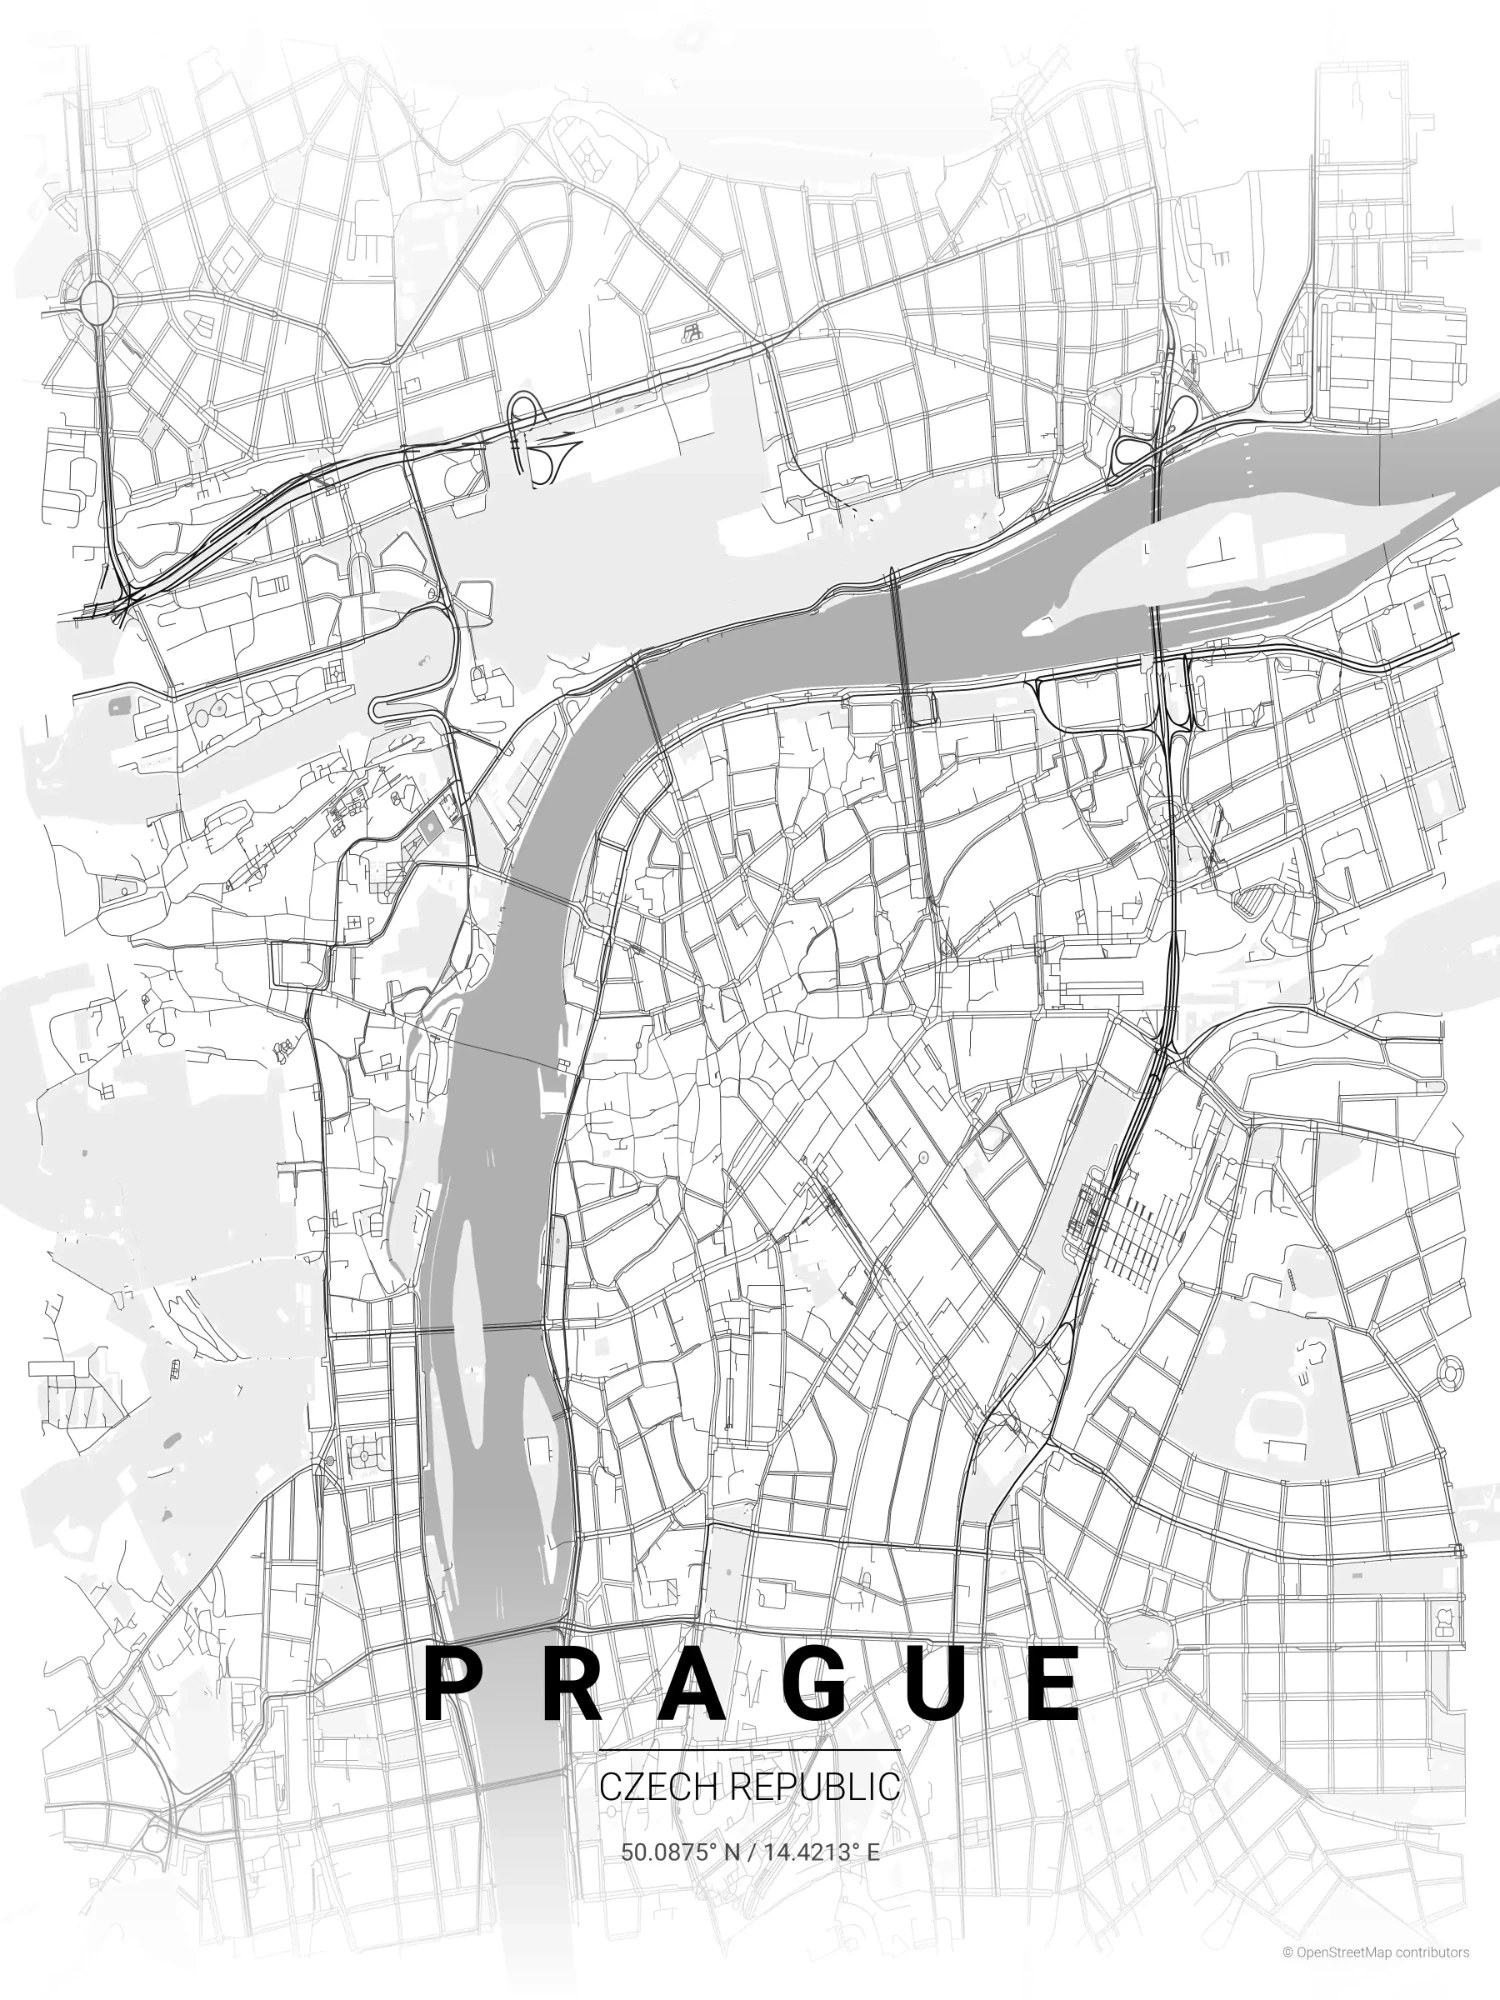
\includegraphics[height=0.80\textheight]{prague_map.jpg}

{\tiny Map data \textcopyright\ OpenStreetMap contributors}
\column{0.56\textwidth}
\begin{itemize}
  \item The Orloj, the astronomical clock on the Old Town Square, is near the centre of the map
  \item East--west distance: how far a caf\'e lies to the left or right of it
  \item North--south distance: how far it lies above or below it
  \item A3 asks which of the two is larger for a typical caf\'e
\end{itemize}
\end{columns}
\end{frame}

%% -------------------------------------------------------------------
\begin{frame}{A3: Caf\'es spread farther east--west than north--south}
\researchq{Are caf\'es spread farther east--west (longitude) than north--south (latitude) from the Orloj?}

\begin{columns}[c]
\column{0.55\textwidth}
\includegraphics[width=\linewidth]{\fig{A3_figure.pdf}}
\column{0.43\textwidth}
\begin{itemize}
  \item Mean difference 0.42 km, 95\% CI [0.28, 0.56], $n = 189$
  \item Effect size: Cohen's $d_z = 0.43$
  \item Paired $t$-test, one-tailed: $t(188) = 5.97$, $p < .001$
\end{itemize}
\begin{block}{In plain words}
A typical caf\'e is about 0.4 km farther from the Orloj east--west than north--south.
\end{block}
\end{columns}
\end{frame}

%% -------------------------------------------------------------------
\begin{frame}{A4: No clear difference in distance between caf\'e types}
\researchq{Does the distance from the Orloj differ by Caf\'e Type (independent, local chain, international chain), and if so, how?}

\begin{columns}[c]
\column{0.50\textwidth}
\includegraphics[width=\linewidth]{\fig{A4_figure.pdf}}
\column{0.48\textwidth}
% The medians and their bootstrapped 95% intervals, exported by 03_analysis.R
\resizebox{\linewidth}{!}{\input{\tab{A4_groups.tex}}}
\begin{itemize}
  \item Kruskal--Wallis test: $H(2) = 4.81$, $p = .090$, $n = 188$
\end{itemize}
\begin{block}{In plain words}
International chains look more central, but with only nine of them there is no evidence of a difference.
\end{block}
\end{columns}
\end{frame}

%% -------------------------------------------------------------------
\begin{frame}{A5: International chains are more often in Prague 1}
\researchq{Is an international chain more likely to be in Prague 1 than other caf\'e types, and if so, by how many percentage points?}

\begin{columns}[c]
\column{0.55\textwidth}
\includegraphics[width=\linewidth]{\fig{A5_figure.pdf}}
\column{0.43\textwidth}
\begin{itemize}
  \item In Prague 1: 6 of 9 international chains (66.67\%), 58 of 179 other caf\'es (32.40\%)
  \item Difference 34.26 percentage points, 95\% CI [2.71, 65.82]
  \item Effect size: Cram\'er's $V = 0.15$
  \item Fisher's exact test, one-tailed: $p = .043$
\end{itemize}
\begin{block}{In plain words}
International chains are about 34 percentage points more likely to be in Prague 1, but nine chains make this very imprecise.
\end{block}
\end{columns}
\end{frame}

%% ===================================================================
%%  PART 2: how busy cafes are (A6 to A10)
%% ===================================================================
\section{Part 2: How busy they are}
\partslide{Part 2: How busy they are}{Questions A6 to A10}{Jaxson Sachs}

%% -------------------------------------------------------------------
\begin{frame}{A6: Caf\'es farther from the Orloj have fewer ratings}
\researchq{Is the number of Google ratings correlated with the distance from the Orloj, and if so, in which direction and how strongly?}

\begin{columns}[c]
\column{0.55\textwidth}
\includegraphics[width=\linewidth]{\fig{A6_figure.pdf}}
\column{0.43\textwidth}
\begin{itemize}
  \item Spearman's $\rho = -0.33$, 95\% CI [$-0.46$, $-0.19$], $n = 187$
  \item Effect size: $\rho^2 = 0.11$
  \item Spearman correlation test: $p < .001$
\end{itemize}
\begin{block}{In plain words}
A moderate negative link: the farther a caf\'e is from the Orloj, the fewer ratings it tends to have.
\end{block}
\end{columns}
\end{frame}

%% -------------------------------------------------------------------
\begin{frame}{A7: About 330 fewer ratings for each km from the Orloj}
\researchq{By how many ratings does the number of Google ratings change per km from the Orloj?}

\begin{columns}[c]
\column{0.55\textwidth}
\includegraphics[width=\linewidth]{\fig{A7_figure.pdf}}
\column{0.43\textwidth}
\begin{itemize}
  \item Slope $-327.14$ ratings per km, 95\% CI [$-548.43$, $-105.84$], $n = 187$
  \item Effect size: $R^2 = 0.04$
  \item Simple regression: $t = -2.90$, $p = .004$
\end{itemize}
\begin{block}{In plain words}
Each extra km goes with about 327 fewer ratings, but distance explains only 4\% of the differences between caf\'es.
\end{block}
\end{columns}
\end{frame}

%% -------------------------------------------------------------------
\begin{frame}{A8: The link holds for caf\'es of the same size}
\researchq{Does the link between distance from the Orloj and the number of ratings hold once you account for the number of seats inside, and if so, how much of it remains?}

\begin{columns}[c]
\column{0.55\textwidth}
\includegraphics[width=\linewidth]{\fig{A8_figure.pdf}}
\column{0.43\textwidth}
\begin{itemize}
  \item Slope $-229.29$ ratings per km, 95\% CI [$-408.67$, $-49.91$], $n = 187$
  \item 70.09\% of the slope from A7 remains
  \item Effect size: $R^2 = 0.33$
  \item Multiple regression: $t = -2.51$, $p = .013$
\end{itemize}
\begin{block}{In plain words}
Comparing caf\'es with the same number of seats, each extra km still goes with about 229 fewer ratings.
\end{block}
\end{columns}
\end{frame}

%% -------------------------------------------------------------------
\begin{frame}{A9: No evidence that the link differs east and west}
\researchq{Does the relationship between distance from the Orloj and the number of ratings differ between caf\'es east and west of the Orloj, and if so, how?}

\begin{columns}[c]
\column{0.55\textwidth}
\includegraphics[width=\linewidth]{\fig{A9_figure.pdf}}
\column{0.43\textwidth}
\begin{itemize}
  \item Slope $-683.92$ ratings per km in the west, $-206.58$ in the east
  \item Difference between the slopes 477.34, 95\% CI [$-231.32$, 1186.00], $n = 187$
  \item Effect size: $R^2 = 0.06$
  \item Regression with interaction: $t = 1.32$, $p = .188$
\end{itemize}
\begin{block}{In plain words}
The drop looks steeper in the west, but the interval includes zero, so there is no evidence of a difference.
\end{block}
\end{columns}
\end{frame}

%% -------------------------------------------------------------------
\begin{frame}{A10: Each km lowers the chance of being a busy caf\'e by 13 points}
\researchq{Does the probability that a caf\'e has an above-median number of ratings change with each additional km away from the Orloj, and if so, by how many percentage points?}

\begin{columns}[c]
\column{0.55\textwidth}
\includegraphics[width=\linewidth]{\fig{A10_figure.pdf}}
\column{0.43\textwidth}
\begin{itemize}
  \item Average marginal effect $-13.15$ percentage points per km, 95\% CI [$-18.02$, $-8.29$], $n = 187$
  \item Odds ratio 0.55 per km
  \item Logistic regression: $z = -5.30$, $p < .001$
\end{itemize}
\begin{block}{In plain words}
On average, each extra km from the Orloj goes with a 13 percentage point lower chance of having more ratings than the median caf\'e.
\end{block}
\end{columns}
\end{frame}

%% -------------------------------------------------------------------
%% The conclusion is split in two, one slide per presenter.
\begin{frame}{Conclusion, part 1: where caf\'es are}
\textbf{What we found}
\begin{itemize}
  \item The average caf\'e is about 2 km from the Orloj (A1)
  \item Caf\'es spread farther east--west than north--south, by about 0.4 km (A3)
  \item Roasteries may be about half a kilometre farther out, but the evidence is weak (A2)
  \item International chains look more central and are more often in Prague 1, by about 34 percentage points (A4, A5)
\end{itemize}
\textbf{What to keep in mind}
\begin{itemize}
  \item Only 22 roasteries and 9 international chains, so these comparisons are very imprecise
  \item Caf\'es were chosen by students, not at random, so the results describe this sample
\end{itemize}
\end{frame}

%% -------------------------------------------------------------------
\begin{frame}{Conclusion, part 2: how busy they are}
\textbf{What we found}
\begin{itemize}
  \item Caf\'es farther from the Orloj have fewer ratings, also when they have the same number of seats
  \item No evidence that this differs between east and west
\end{itemize}
\textbf{What to keep in mind}
\begin{itemize}
  \item The data are observational, so distance is linked to popularity but not shown to cause it
  \item A few very popular central caf\'es have a large influence on the regression slopes
\end{itemize}
\end{frame}

%% -------------------------------------------------------------------
%% Backup slide for questions: the summary table exported by 03_analysis.R
\begin{frame}{Backup: all ten results}
\centering
\resizebox{\textwidth}{!}{\input{\tab{summary.tex}}}

\medskip
{\footnotesize CI is the 95\% confidence interval, two-sided also for the one-tailed tests. pp = percentage points.}
\end{frame}

\end{document}
